% Đề thi giữa kỳ CSDL (INT1313) — Lớp tài năng ATTT — Mã đề 104
% Tái tạo từ ảnh chụp đề in (trang 1–3). Trang 4–7 (giấy nháp, phiếu trả lời) không có ảnh,
% được dựng lại theo "Quy định trình bày" của đề.
% Biên dịch (trong thư mục nguon/): xelatex DeGiuaKy_CSDL_MaDe104.tex
% Sơ đồ ER nằm ở SoDoER_MaDe104.tex; SoDoER_standalone.tex xuất riêng hình cho bản Word.
\documentclass[11pt,a4paper]{article}
\usepackage[a4paper,top=2.1cm,bottom=2.0cm,left=1.9cm,right=1.9cm,headheight=13pt,headsep=12pt,footskip=26pt]{geometry}
\usepackage{amsmath}
\usepackage{fontspec}
\usepackage{unicode-math}
\setmainfont{Latin Modern Roman}[SmallCapsFont={Latin Modern Roman Caps}]
\setmonofont{Latin Modern Mono}
\setmathfont{Latin Modern Math}
\usepackage{fancyhdr}
\usepackage{array}
\usepackage{booktabs}
\usepackage{enumitem}
\usepackage{tikz}
\usetikzlibrary{shapes.geometric,calc}

\hyphenpenalty=10000
\exhyphenpenalty=10000
\setlength{\parindent}{0pt}
\setlength{\parskip}{0pt}

\newcommand{\made}{104}
\pagestyle{fancy}
\fancyhf{}
\fancyhead[L]{\small CSDL INT1313\qquad Mã đề \made}
\fancyhead[R]{\small Giữa kỳ — Lớp tài năng ATTT}
\fancyfoot[C]{Trang \thepage/7 — Mã đề \made}
\renewcommand{\headrulewidth}{0.4pt}

% Tên quan hệ, thuộc tính, hằng: chữ máy chữ
\newcommand{\tn}[1]{\texttt{#1}}
% Tiêu đề phần
\newcommand{\phan}[4][]{\par\bigskip{\large\textbf{PHẦN #2.\ \ #3} \textit{(#4)}#1}\par\smallskip}
% Câu trắc nghiệm
\newcommand{\cau}[2]{\par\textbf{#1.} #2\par}
\newlist{pa}{enumerate}{1}
\setlist[pa]{label=\Alph*.,leftmargin=3.2em,labelsep=0.45em,itemsep=0pt,parsep=0pt,topsep=0pt,partopsep=0pt,before={\vspace{0.75\baselineskip}\small}}
\newcommand{\pangang}[1]{\par{\small\hspace*{2.1em}#1\par}}
\newcommand{\ghichu}[1]{\par{\footnotesize #1}\par}
\newcommand{\hop}[1]{\fbox{\normalsize\rmfamily #1}}

\begin{document}

% ============================== TRANG 1 ==============================
\begin{center}
\textsc{Học Viện Công Nghệ Bưu Chính Viễn Thông — Khoa Trí Tuệ Nhân Tạo}\\[1pt]
{\Large\bfseries ĐỀ THI GIỮA KỲ — CƠ SỞ DỮ LIỆU (INT1313)}\\[3pt]
Lớp tài năng ngành An toàn thông tin \quad — \quad \textbf{M{\small Ã} Đ{\small Ề} 104}\\[1pt]
\textbf{Thời gian: 90 phút\enspace|\enspace Không sử dụng tài liệu\enspace|\enspace Thang điểm 10}
\end{center}
\vspace{-4pt}
\rule{\textwidth}{0.6pt}\par\smallskip

{\large\bfseries QUY ĐỊNH TRÌNH BÀY}\par\smallskip
\begin{enumerate}[label=\arabic*.,leftmargin=*,itemsep=1pt,parsep=0pt,topsep=0pt]
\item \textbf{Chỉ PHIẾU TRẢ LỜI (2 trang cuối, in 2 mặt) được chấm.} Đáp án viết trên phần đề hoặc giấy nháp không được tính điểm.
\item \textbf{Tập thuộc tính viết liền, theo thứ tự bảng chữ cái:} viết {\small\textsf{ABCD}}, không viết $\{B,A,D,C\}$.
\item \textbf{Mỗi ô một đáp án.} Ô có hai đáp án hoặc tẩy xóa không rõ tính là \textbf{sai}.
\item Phần F trả lời trong khung: \textbf{F1 tối đa 3 dòng, F2 tối đa 4 dòng}; ngoài khung không chấm.
\item \textbf{Không dùng bút chì} cho phiếu trả lời.
\end{enumerate}
\vspace{2pt}
\rule{\textwidth}{0.6pt}

\phan[\ \textbf{— 12 câu, mỗi câu 0,15}]{A}{Trắc nghiệm}{1,8 điểm}
\ghichu{Mỗi câu có ba phương án; chọn một và điền vào phiếu trả lời.}

\cau{1}{Khi chuyển liên kết M:N có thuộc tính riêng sang mô hình quan hệ, khóa chính là:}
\begin{pa}
\item một trong hai khóa ngoại
\item hợp của hai khóa ngoại
\item hợp của hai khóa ngoại và các thuộc tính riêng
\end{pa}

\cau{2}{Thuật toán phân rã BCNF bảo đảm tính chất nào?}
\pangang{A.~cả hai.\qquad B.~chỉ bảo toàn phụ thuộc.\qquad C.~chỉ kết nối không mất mát.}

\cau{3}{$Z$ phụ thuộc bắc cầu vào $X$ khi $X\to Y, Y\to Z$ và \textbf{thêm điều kiện}:}
\begin{pa}
\item không cần thêm điều kiện nào
\item $Y\nrightarrow X$ và $Z\notin X\cup Y$
\item $Y$ phải là thuộc tính khóa
\end{pa}

\cau{4}{$K$ là khóa ứng viên của $R$ khi $\{K\}^+=R$ và:}
\begin{pa}
\item $K$ là duy nhất
\item không tập con nào của $K$ là siêu khóa
\item không tập con \textit{thực sự} nào của $K$ là siêu khóa
\end{pa}

\cau{5}{Cho $R(A,B,C)$ với $F=\{A\to B,\ B\to C\}$. Khi đó $R$:}
\pangang{A.~đạt 2NF nhưng không đạt 3NF.\qquad B.~đạt 3NF.\qquad C.~không đạt 2NF.}

\cau{6}{Quy tắc suy diễn nào sau đây \textbf{KHÔNG} đúng?}
\begin{pa}
\item nếu $XY\to Z$ thì $X\to Z$
\item nếu $X\to Y$ và $Y\to Z$ thì $X\to Z$
\item nếu $X\to YZ$ thì $X\to Y$
\end{pa}

\cau{7}{Mọi lược đồ quan hệ chỉ có \textbf{hai} thuộc tính thì:}
\pangang{A.~luôn đạt 3NF nhưng chưa chắc BCNF.\qquad B.~luôn đạt BCNF.\qquad C.~có thể không đạt 2NF.}

\cau{8}{Phân rã $R$ thành $R_1, R_2$ là \textit{không mất mát} khi và chỉ khi:}
\begin{pa}
\item $R_1\cap R_2$ là siêu khóa của cả hai quan hệ con
\item $R_1\cap R_2$ là siêu khóa của ít nhất một quan hệ con
\item $R_1\cap R_2\neq\varnothing$
\end{pa}

\cau{9}{Nếu một phân rã nhị phân là không mất mát thì:}
\begin{pa}
\item nó cũng bảo toàn phụ thuộc
\item nó chắc chắn không bảo toàn phụ thuộc
\item chưa kết luận được gì về bảo toàn phụ thuộc
\end{pa}

\newpage
% ============================== TRANG 2 ==============================
\cau{10}{Một thể hiện cụ thể của $R$ thỏa mãn $X\to Y$. Kết luận đúng là:}
\pangang{A.~chưa kết luận được gì.\qquad B.~$X$ là siêu khóa của $R$.\qquad C.~$X\to Y$ là phụ thuộc hàm của lược đồ.}

\cau{11}{Phép chiếu tập phụ thuộc hàm $\pi_S(F)$ xuống tập thuộc tính $S$:}
\begin{pa}
\item có thể chứa phụ thuộc không xuất hiện trong $F$
\item chỉ gồm các phụ thuộc của $F$ có cả hai vế nằm trong $S$
\item luôn rỗng nếu $S$ không chứa khóa nào của $R$
\end{pa}

\cau{12}{Trong một lược đồ quan hệ bất kỳ, thuộc tính $H$ không xuất hiện ở vế trái lẫn vế phải của phụ thuộc hàm nào. Khi đó $H$:}
\begin{pa}
\item có thể thuộc hoặc không thuộc khóa, tùy vào $F$
\item không thuộc khóa ứng viên nào
\item thuộc mọi khóa ứng viên
\end{pa}

\phan{B}{Phụ thuộc hàm}{2,8 điểm}
Cho $R(A,B,C,D,E,G)$ và $F=\{\,AD\to B,\quad B\to D,\quad BG\to E,\quad E\to DG\,\}$\par\smallskip
\textbf{B1. Bao đóng} \textit{(0,8 điểm)} — tính và điền vào phiếu: $\{B\}^+$,\ \ $\{AB\}^+$,\ \ $\{ACE\}^+$,\ \ $\{ABC\}^+$ (lần lượt là ô B1a, B1b, B1c, B1d).\par\smallskip
\textbf{B2. Phân loại} \textit{(1,2 điểm)} — với mỗi tập, điền \textbf{K} (là khóa ứng viên) / \textbf{S} (là siêu khóa nhưng không tối thiểu) / \textbf{N} (không phải siêu khóa):\par\smallskip
\begin{center}
\renewcommand{\arraystretch}{1.15}
\begin{tabular}{|c|*{8}{>{\centering\arraybackslash}p{1.25cm}|}}
\hline
\textbf{Ô} & \textbf{B2a} & \textbf{B2b} & \textbf{B2c} & \textbf{B2d} & \textbf{B2e} & \textbf{B2f} & \textbf{B2g} & \textbf{B2h}\\\hline
\textbf{Tập} & $ABCE$ & $ACE$ & $ABCD$ & $ABCG$ & $ABC$ & $ABD$ & $ACDG$ & $ACDE$\\\hline
\end{tabular}
\end{center}
\vspace{-6pt}
\ghichu{\textit{Tính điểm:} đúng cả $8=1{,}2$; sai 1–2 ô $=0{,}6$; sai từ 3 ô $=0$.}
\smallskip
\textbf{B3. Phủ tối thiểu} \textit{(0,8 điểm)} — khoanh vào phiếu những số thuộc phủ tối thiểu của $F$. \textit{(Với tập $F$ này phủ tối thiểu là duy nhất.)}\par
\begin{center}
\begin{tabular}{lllll}
\toprule
1. $E\to DG$ & 3. $AB\to D$ & 5. $B\to D$ & 7. $BG\to E$ & 9. $G\to C$\\
2. $AD\to B$ & 4. $AE\to B$ & 6. $G\to B$ & 8. $E\to D$ & 10. $E\to G$\\
\bottomrule
\end{tabular}
\end{center}
\vspace{-6pt}
\ghichu{\textit{Lưu ý:} trong danh sách có phụ thuộc \textit{suy diễn được} từ $F$ nhưng \textit{không} thuộc phủ tối thiểu, và có cả phụ thuộc không suy diễn được từ $F$. \textit{Tính điểm:} đúng hoàn toàn $=0{,}8$; mỗi số thừa hoặc thiếu trừ $0{,}2$; tối thiểu 0.}

\phan{C}{Phân rã}{2,0 điểm}
\textbf{C1} \textit{(1,2 điểm)} — Cho $R(A,B,C,D)$ và $F=\{\,A\to B,\quad BD\to A\,\}$. Với mỗi phép phân rã, điền \textbf{Đ/S} cho hai câu hỏi độc lập:\par
\begin{center}
\renewcommand{\arraystretch}{1.15}
\begin{tabular}{|l|p{3.1cm}|p{3.6cm}|p{4.2cm}|}
\hline
\textbf{Ô} & \textbf{Phép phân rã} & \textbf{Không mất mát?} & \textbf{Bảo toàn phụ thuộc?}\\\hline
C1a & $\{ABD,\ ACD\}$ & & \\\hline
C1b & $\{AB,\ ACD\}$ & & \\\hline
C1c & $\{AC,\ ABD\}$ & & \\\hline
C1d & $\{AB,\ CD\}$ & & \\\hline
\end{tabular}
\end{center}
\vspace{-6pt}
\ghichu{Mỗi ô 0,15 điểm (8 ô). Hai cột chấm độc lập — phải điền cả hai cột cho mỗi phép phân rã; bỏ trống tính sai.}
\smallskip
\textbf{C2} \textit{(0,8 điểm)} — Quay lại lược đồ $R(A,B,C,D,E,G)$ ở Phần B. Xét phép chiếu $\pi_{ABDE}(F)$. Với mỗi phụ thuộc dưới đây, điền \textbf{Đ} nếu nó \textit{suy diễn được} từ $F$ (tức thuộc $\pi_{ABDE}(F)$), \textbf{S} nếu không:\par
\begin{center}
\renewcommand{\arraystretch}{1.15}
\begin{tabular}{|c|*{8}{w{c}{1.3cm}|}}
\hline
\textbf{Ô} & \textbf{C2a} & \textbf{C2b} & \textbf{C2c} & \textbf{C2d} & \textbf{C2e} & \textbf{C2f} & \textbf{C2g} & \textbf{C2h}\\\hline
\textbf{FD} & $A\to E$ & $AE\to B$ & $B\to D$ & $B\to A$ & $E\to D$ & $B\to E$ & $D\to A$ & $AB\to D$\\\hline
\end{tabular}
\end{center}
\vspace{-6pt}
\ghichu{Mỗi ô 0,1 điểm; bỏ trống tính sai.}

\newpage
% ============================== TRANG 3 ==============================
\phan{D}{Mô hình thực thể — liên kết}{1,2 điểm}
\begin{center}
% Sơ đồ ER Phần D, mã đề 104. Toạ độ đo trên ảnh chụp đề gốc (đơn vị: pixel ảnh).
% Vẽ ở cỡ lớn rồi thu nhỏ 0,65 lần, giống cách đề gốc thu nhỏ hình.
\scalebox{0.65}{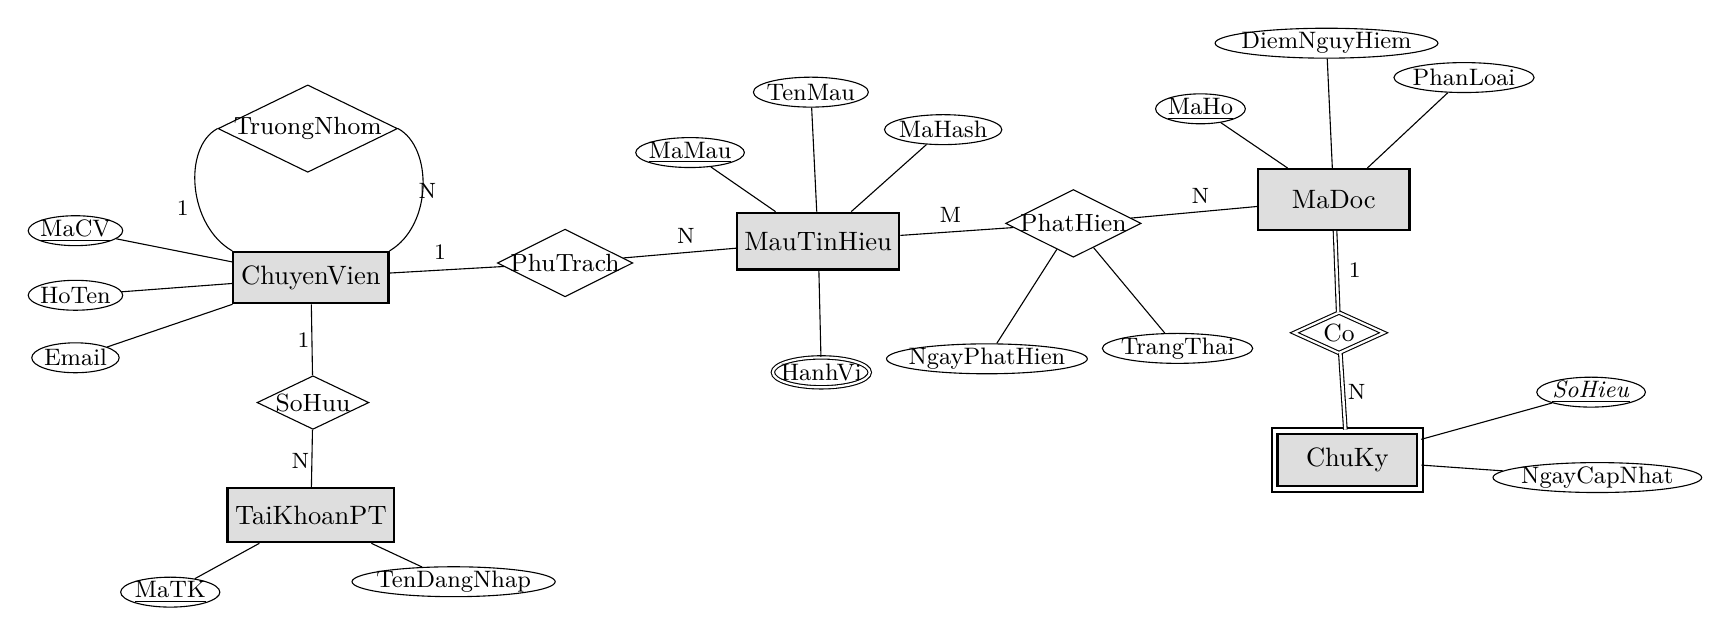
\begin{tikzpicture}[x=0.01323cm,y=-0.01323cm,font=\fontsize{9.6}{11}\selectfont,
  ent/.style={draw,thick,fill=black!13,inner sep=0pt},
  rel/.style={draw,diamond,fill=white,inner sep=0pt},
  att/.style={draw,ellipse,fill=white,inner sep=0pt,minimum height=0.38cm},
  every label/.style={font=\fontsize{8.6}{10}\selectfont,inner sep=0pt},
  card/.style={font=\fontsize{8}{9}\selectfont,inner sep=1pt}]
% Toạ độ đo trực tiếp trên ảnh chụp (đơn vị: pixel ảnh)
% --- ChuyenVien, TruongNhom (đệ quy), SoHuu, TaiKhoanPT
\node[ent,minimum width=1.97cm,minimum height=0.65cm] (cv) at (513,300) {ChuyenVien};
\node[rel,minimum width=2.28cm,minimum height=1.11cm,shape aspect=2.06,label={[font=\fontsize{9}{10}\selectfont]center:TruongNhom}] (tn) at (510,157) {};
\node[att,minimum width=1.20cm,label={center:\underline{MaCV}}] (macv) at (287,255) {};
\node[att,minimum width=1.20cm,label={center:HoTen}] (hoten) at (287,317) {};
\node[att,minimum width=1.11cm,label={center:Email}] (email) at (287,377) {};
\draw (macv) -- (cv); \draw (hoten) -- (cv); \draw (email) -- (cv);
\draw (cv.north west) .. controls (395,250) and (390,175) .. (tn.west);
\draw (cv.north east) .. controls (630,250) and (630,175) .. (tn.east);
\node[card] at (390,233) {1};
\node[card] at (625,217) {N};
\node[rel,minimum width=1.42cm,minimum height=0.68cm,shape aspect=2.09,label={[font=\fontsize{9}{10}\selectfont]center:SoHuu}] (sh) at (515,420) {};
\node[ent,minimum width=2.12cm,minimum height=0.69cm] (tk) at (513,528) {TaiKhoanPT};
\draw (cv) -- (sh); \draw (sh) -- (tk);
\node[card] at (506,360) {1};
\node[card] at (503,476) {N};
\node[att,minimum width=1.26cm,label={center:\underline{MaTK}}] (matk) at (378,602) {};
\node[att,minimum width=2.58cm,label={center:TenDangNhap}] (tdn) at (650,592) {};
\draw (matk) -- (tk); \draw (tdn) -- (tk);
% --- PhuTrach, MauTinHieu
\node[rel,minimum width=1.72cm,minimum height=0.86cm,shape aspect=2.00,label={[font=\fontsize{9}{10}\selectfont]center:PhuTrach}] (pt) at (757,286) {};
\node[ent,minimum width=2.06cm,minimum height=0.72cm] (mth) at (1000,265) {MauTinHieu};
\draw (cv) -- (pt); \draw (pt) -- (mth);
\node[card] at (637,276) {1};
\node[card] at (873,260) {N};
\node[att,minimum width=1.38cm,label={center:\underline{MaMau}}] (mamau) at (877,180) {};
\node[att,minimum width=1.46cm,label={center:TenMau}] (tenmau) at (993,122) {};
\node[att,minimum width=1.49cm,label={center:MaHash}] (mahash) at (1120,158) {};
\draw (mamau) -- (mth); \draw (tenmau) -- (mth); \draw (mahash) -- (mth);
\node[att,double,double distance=0.8pt,minimum width=1.23cm,label={center:HanhVi}] (hv) at (1003,391) {};
\draw (mth) -- (hv);
% --- PhatHien (M:N), MaDoc
\node[rel,minimum width=1.72cm,minimum height=0.86cm,shape aspect=2.00,label={[font=\fontsize{9}{10}\selectfont]center:PhatHien}] (ph) at (1245,248) {};
\node[ent,minimum width=1.92cm,minimum height=0.77cm] (md) at (1495,225) {MaDoc};
\draw (mth) -- (ph); \draw (ph) -- (md);
\node[card] at (1127,240) {M};
\node[card] at (1367,222) {N};
\node[att,minimum width=2.55cm,label={center:NgayPhatHien}] (nph) at (1162,378) {};
\node[att,minimum width=1.91cm,label={center:TrangThai}] (tt) at (1345,368) {};
\draw (ph) -- (nph); \draw (ph) -- (tt);
\node[att,minimum width=1.14cm,label={center:\underline{MaHo}}] (maho) at (1367,138) {};
\node[att,minimum width=2.83cm,label={center:DiemNguyHiem}] (dnh) at (1488,75) {};
\node[att,minimum width=1.78cm,label={center:PhanLoai}] (pl) at (1620,108) {};
\draw (maho) -- (md); \draw (dnh) -- (md); \draw (pl) -- (md);
% --- Co (liên kết định danh), ChuKy (thực thể yếu)
\node[rel,double,double distance=0.8pt,minimum width=1.14cm,minimum height=0.52cm,shape aspect=2.18,label={[font=\fontsize{9}{10}\selectfont]center:Co}] (co) at (1500,353) {};
\node[ent,double,double distance=1.3pt,minimum width=1.85cm,minimum height=0.74cm] (ck) at (1508,475) {ChuKy};
\draw[double,double distance=0.9pt] (md) -- (co);
\draw[double,double distance=0.9pt] (co) -- (ck);
\node[card] at (1515,293) {1};
\node[card] at (1517,410) {N};
\node[att,minimum width=1.38cm,label={center:\underline{\textit{SoHieu}}}] (sohieu) at (1742,410) {};
\node[att,minimum width=2.65cm,label={center:NgayCapNhat}] (ncn) at (1748,492) {};
\draw (ck) -- (sohieu); \draw (ck) -- (ncn);
\end{tikzpicture}}

\end{center}
\vspace{-2pt}
{\footnotesize Chữ nhật nét đôi = thực thể yếu; thoi nét đôi = liên kết định danh; bầu dục nét đôi = thuộc tính đa trị; gạch chân = khóa chính; gạch chân \textit{nghiêng} = khóa bộ phận.\par
\textbf{Quy ước đặt tên khóa ngoại:} khóa ngoại sinh ra từ liên kết đệ quy \tn{TruongNhom} đặt tên \tn{MaTruongNhom}; khóa ngoại sinh ra từ liên kết \tn{PhuTrach} đặt tên \tn{MaCVPhuTrach}.\par}
Dưới đây là 8 quan hệ ứng viên. Điền \textbf{Đ} nếu quan hệ thuộc lược đồ đúng, \textbf{S} nếu không; nếu \textbf{Đ} thì ghi thêm \textbf{khóa chính}.\par
\begin{center}\small
\begin{tabular}{ll}
\toprule
\textbf{Ô} & \textbf{Quan hệ ứng viên}\\
\midrule
D1 & \tn{ChuyenVien(MaCV, HoTen, Email, MaTruongNhom, MaTK, TenDangNhap)}\\
D2 & \tn{ChuKy(SoHieu, NgayCapNhat)}\\
D3 & \tn{MauTinHieu\_HanhVi(MaMau, HanhVi)}\\
D4 & \tn{ChuyenVien(MaCV, HoTen, Email, MaTruongNhom)}\\
D5 & \tn{PhatHien(MaMau, MaHo, NgayPhatHien, TrangThai)}\\
D6 & \tn{TaiKhoanPT(MaTK, TenDangNhap, MaCV)}\\
D7 & \tn{MaDoc(MaHo, DiemNguyHiem, PhanLoai)}\\
D8 & \tn{MauTinHieu(MaMau, TenMau, MaHash, HanhVi, MaCVPhuTrach)}\\
\bottomrule
\end{tabular}
\end{center}
\vspace{-6pt}
\ghichu{Mỗi ô đúng cả Đ/S và khóa chính $=0{,}15$ điểm.}

\phan{E}{Đại số quan hệ}{1,0 điểm}
Dùng ba quan hệ:\par
\begin{itemize}[leftmargin=2.2em,itemsep=0pt,parsep=0pt,topsep=0pt,label=\textbullet]\small
\item \tn{MauTinHieu(\underline{MaMau}, ..., MaHash)}
\item \tn{MaDoc(\underline{MaHo}, ..., PhanLoai)}
\item \tn{PhatHien(\underline{\textit{MaMau}}, \underline{\textit{MaHo}}, TrangThai)}
\end{itemize}
\textbf{E1–E3.} Giá trị \tn{MaHash} của những mẫu tín hiệu có ít nhất một họ mã độc mức \tn{’APT’} ở trạng thái \tn{\textit{’CHUA\_CACH\_LY’}}:
\[
\pi_{\hop{E1}}\Bigl(\tn{MauTinHieu}\bowtie\bigl(\sigma_{\hop{E2}}(\tn{PhatHien})\bowtie\sigma_{\hop{E3}}(\tn{MaDoc})\bigr)\Bigr)
\]
\textbf{E4.} Mã những mẫu tín hiệu \textbf{không} có họ mã độc nào mức \tn{’APT’}:
\[
\pi_{\tn{MaMau}}\bigl(\tn{MauTinHieu}\bigr)\ \ \hop{E4}\ \ \pi_{\tn{MaMau}}\bigl(\tn{PhatHien}\bowtie\sigma_{\tn{PhanLoai=’APT’}}(\tn{MaDoc})\bigr)
\]
\textbf{E5.} Mã những mẫu tín hiệu bị ảnh hưởng bởi \textbf{mọi} họ mã độc mức \tn{’APT’}:
\[
\pi_{\tn{MaMau, MaHo}}\bigl(\tn{PhatHien}\bigr)\ \ \hop{E5}\ \ \pi_{\tn{MaHo}}\bigl(\sigma_{\tn{PhanLoai=’APT’}}(\tn{MaDoc})\bigr)
\]
\ghichu{\textit{Mỗi ô 0,2 điểm.} Ô E1–E3 điền danh sách thuộc tính hoặc điều kiện; ô E4, E5 điền \textit{một toán tử}.}

\phan{F}{Tự luận ngắn}{1,2 điểm}
Vẫn dùng $R(A,B,C,D)$ với $F=\{\,A\to B,\quad BD\to A\,\}$ ở Phần C.\par\smallskip
\textbf{F1} \textit{(0,6 điểm)} Chứng minh $R$ \textbf{đạt 3NF}. Yêu cầu: nêu đủ các khóa ứng viên, tập thuộc tính khóa, rồi xét từng phụ thuộc hàm. \textit{(Tối đa 3 dòng)}\par\smallskip
\textbf{F2} \textit{(0,6 điểm)} $R$ có đạt BCNF không? Nếu không, hãy làm đủ ba việc: \textbf{(a)} chỉ rõ các phụ thuộc vi phạm; \textbf{(b)} phân rã $R$ về BCNF và viết các lược đồ con thu được; \textbf{(c)} chỉ rõ phụ thuộc hàm nào \textit{bị mất} sau phân rã. \textit{(Tối đa 4 dòng)}

\newpage
% ============================== TRANG 4–5: GIẤY NHÁP ==============================
\begin{center}
{\large\bfseries GIẤY NHÁP}\\[2pt]
{\small\itshape Phần viết ở đây không được chấm.}
\end{center}
\null\newpage
\begin{center}
{\large\bfseries GIẤY NHÁP}\\[2pt]
{\small\itshape Phần viết ở đây không được chấm.}
\end{center}
\null\newpage

% ============================== TRANG 6–7: PHIẾU TRẢ LỜI ==============================
\newcommand{\dong}[1]{\makebox[#1]{\dotfill}}
\newcommand{\phieuphan}[2]{\par\medskip{\bfseries PHẦN #1.\ \ #2}\par\smallskip}
\renewcommand{\arraystretch}{1.6}

\begin{center}
{\LARGE\bfseries PHIẾU TRẢ LỜI}\\[2pt]
Đề thi giữa kỳ — Cơ sở dữ liệu (INT1313) \quad — \quad \textbf{M{\small Ã} Đ{\small Ề} 104}
\end{center}
Họ và tên: \dong{6.0cm}\quad Mã sinh viên: \dong{3.0cm}\quad Lớp: \dong{2.0cm}\par
\vspace{2pt}\rule{\textwidth}{0.6pt}

\phieuphan{A}{Trắc nghiệm \textmd{\textit{(1,8 điểm) — ghi A, B hoặc C}}}
\begin{center}
\begin{tabular}{|>{\bfseries}c|*{12}{>{\centering\arraybackslash}p{0.82cm}|}}
\hline
Câu & \textbf{1} & \textbf{2} & \textbf{3} & \textbf{4} & \textbf{5} & \textbf{6} & \textbf{7} & \textbf{8} & \textbf{9} & \textbf{10} & \textbf{11} & \textbf{12}\\\hline
Đáp án & & & & & & & & & & & & \\\hline
\end{tabular}
\end{center}

\phieuphan{B}{Phụ thuộc hàm \textmd{\textit{(2,8 điểm)}}}
\textbf{B1. Bao đóng}\par\smallskip
\begin{center}
\begin{tabular}{|c|p{3.25cm}|c|p{3.25cm}|}
\hline
\textbf{B1a}\ \ $\{B\}^+$ & & \textbf{B1b}\ \ $\{AB\}^+$ & \\\hline
\textbf{B1c}\ \ $\{ACE\}^+$ & & \textbf{B1d}\ \ $\{ABC\}^+$ & \\\hline
\end{tabular}
\end{center}
\textbf{B2. Phân loại} \textit{(ghi K / S / N)}\par\smallskip
\begin{center}
\begin{tabular}{|>{\bfseries}c|*{8}{>{\centering\arraybackslash}p{1.25cm}|}}
\hline
Ô & \textbf{B2a} & \textbf{B2b} & \textbf{B2c} & \textbf{B2d} & \textbf{B2e} & \textbf{B2f} & \textbf{B2g} & \textbf{B2h}\\\hline
Tập & $ABCE$ & $ACE$ & $ABCD$ & $ABCG$ & $ABC$ & $ABD$ & $ACDG$ & $ACDE$\\\hline
K/S/N & & & & & & & & \\\hline
\end{tabular}
\end{center}
\textbf{B3. Phủ tối thiểu} \textit{(khoanh tròn các số thuộc phủ tối thiểu của $F$)}\par\smallskip
\begin{center}
\Large 1\qquad 2\qquad 3\qquad 4\qquad 5\qquad 6\qquad 7\qquad 8\qquad 9\qquad 10
\end{center}

\phieuphan{C}{Phân rã \textmd{\textit{(2,0 điểm) — ghi Đ hoặc S}}}
\textbf{C1}\par\smallskip
\begin{center}
\begin{tabular}{|l|p{3.1cm}|>{\centering\arraybackslash}p{3.6cm}|>{\centering\arraybackslash}p{4.2cm}|}
\hline
\textbf{Ô} & \textbf{Phép phân rã} & \textbf{Không mất mát?} & \textbf{Bảo toàn phụ thuộc?}\\\hline
C1a & $\{ABD,\ ACD\}$ & & \\\hline
C1b & $\{AB,\ ACD\}$ & & \\\hline
C1c & $\{AC,\ ABD\}$ & & \\\hline
C1d & $\{AB,\ CD\}$ & & \\\hline
\end{tabular}
\end{center}
\textbf{C2}\par\smallskip
\begin{center}
\begin{tabular}{|>{\bfseries}c|*{8}{w{c}{1.3cm}|}}
\hline
Ô & \textbf{C2a} & \textbf{C2b} & \textbf{C2c} & \textbf{C2d} & \textbf{C2e} & \textbf{C2f} & \textbf{C2g} & \textbf{C2h}\\\hline
FD & $A\to E$ & $AE\to B$ & $B\to D$ & $B\to A$ & $E\to D$ & $B\to E$ & $D\to A$ & $AB\to D$\\\hline
Đ/S & & & & & & & & \\\hline
\end{tabular}
\end{center}

\newpage
\phieuphan{D}{Mô hình thực thể — liên kết \textmd{\textit{(1,2 điểm)}}}
\begin{center}
\begin{tabular}{|c|>{\centering\arraybackslash}p{1.6cm}|p{10.5cm}|}
\hline
\textbf{Ô} & \textbf{Đ/S} & \textbf{Khóa chính (nếu Đ)}\\\hline
D1 & & \\\hline
D2 & & \\\hline
D3 & & \\\hline
D4 & & \\\hline
D5 & & \\\hline
D6 & & \\\hline
D7 & & \\\hline
D8 & & \\\hline
\end{tabular}
\end{center}

\phieuphan{E}{Đại số quan hệ \textmd{\textit{(1,0 điểm)}}}
\begin{center}
\begin{tabular}{|c|p{13.5cm}|}
\hline
\textbf{E1} & \\\hline
\textbf{E2} & \\\hline
\textbf{E3} & \\\hline
\end{tabular}
\\[6pt]
\begin{tabular}{|c|p{3cm}|c|p{3cm}|}
\hline
\textbf{E4} & & \textbf{E5} & \\\hline
\end{tabular}
\end{center}

\phieuphan{F}{Tự luận ngắn \textmd{\textit{(1,2 điểm)}}}
\newcommand{\khung}[1]{\par\noindent\begin{tikzpicture}
\draw[thick] (0,0) rectangle (\textwidth-0.8pt,-#1*0.85cm-0.25cm);
\foreach \i in {1,...,#1} \draw[gray!70,dotted] (0.2cm,-\i*0.85cm) -- (\textwidth-0.2cm,-\i*0.85cm);
\end{tikzpicture}\par}
\textbf{F1} \textit{(tối đa 3 dòng)}\par\smallskip
\khung{3}\medskip
\textbf{F2} \textit{(tối đa 4 dòng)}\par\smallskip
\khung{4}

\end{document}
